\documentclass[14pt]{extarticle}

\input{metainfo}
\usepackage[T2A]{fontenc}
\usepackage[utf8]{inputenc}
\usepackage[english, russian]{babel}
% \usepackage{cmap}
\usepackage{url}
\usepackage{booktabs}
\usepackage{nicefrac}
\usepackage{microtype}
\usepackage{lipsum}
\usepackage{graphicx}
\usepackage{subfig}
\usepackage[square,sort,comma,numbers]{natbib}
\usepackage{doi}
\usepackage{multicol}
\usepackage{multirow}
\usepackage{tabularx}

\usepackage{tikz}
\usetikzlibrary{matrix}

% Algorithms
\usepackage{algpseudocode}
\usepackage{algorithm}

%% Шрифты
\usepackage{euscript} % Шрифт Евклид
\usepackage{mathrsfs} % Красивый матшрифт
\usepackage{extsizes}

\usepackage{makecell} % diaghead in a table
\usepackage{amsmath,amsfonts,amssymb,amsthm,mathtools,dsfont}
\usepackage{icomma}

\usepackage{hyperref}
% \usepackage[usenames,dvipsnames,svgnames,table,rgb]{xcolor}

\hypersetup{
	unicode=true,
	pdftitle={Multi Objective Lipschitz Competitive Solution Search},
	pdfauthor={Латыпов Ильгам Магданович},
	pdfkeywords={многокритериальная оптимизация, competitive solution},
	colorlinks=true,
	linkcolor=black,        % внутренние ссылки
	citecolor=green,         % на библиографию
	filecolor=magenta,      % на файлы
	urlcolor=blue           % на URL
}

\graphicspath{{figs}}

\usepackage{enumitem} % Для модификаций перечневых окружений
\usepackage{etoolbox}

\makeatletter
\expandafter\patchcmd\csname\string\algorithmic\endcsname{\itemsep\z@}{\itemsep=1.5mm}{}{}
\makeatother

\usepackage{geometry}
\geometry{left=3cm}
\geometry{right=1.5cm}
\geometry{top=2.0cm}
\geometry{bottom=2.0cm}
\setlength\parindent{5ex}    % Устанавливает длину красной строки 15pt
\linespread{1.3}             % Коэффициент межстрочного интервала
\usepackage[center]{titlesec}

\usepackage{icomma}
\usepackage{amsthm}
\usepackage{graphicx}
\usepackage{amssymb}
\usepackage{amsmath}
\usepackage{graphicx}
\usepackage{color}
%\usepackage{bm}
\usepackage{tabularx}
\usepackage{url}
\usepackage{multirow}
\usepackage{wrapfig}
\usepackage{caption}
\usepackage{subcaption}

% Теоремы
\newtheorem{comments}{Комментарий}
\newtheorem{assumption}{Предположения}
\newtheorem{theorem}{Теорема}
\newtheorem{lemma}{Лемма}
\newtheorem{proposition}{Утверждение}
\newtheorem*{exercise}{Упражнение}
\newtheorem*{problem}{Задача}

\newtheorem{definition}{Определение}
\newtheorem*{corollary}{Следствие}
\newtheorem*{note}{Замечание}
\newtheorem*{reminder}{Напоминание}
\newtheorem*{example}{Пример}
\newtheorem*{cexample}{Контрпример}
\newtheorem*{solution}{Решение}
\renewcommand{\abstractname}{Аннотация}

\usepackage{todonotes}
% \documentclass[a4paper,14pt]{extarticle}
\usepackage[utf8]{inputenc}
\usepackage[T1,T2A]{fontenc}
\usepackage[english,russian]{babel}

\usepackage{amsthm}
\usepackage{graphicx}
\usepackage{caption}
\usepackage{amssymb}
\usepackage{amsmath}
\usepackage{mathrsfs}
\usepackage{euscript}
\usepackage{graphicx}
\usepackage{subfig}
\usepackage{caption}
\usepackage{color}
\usepackage{bm}
\usepackage{tabularx}
\usepackage{url}
\usepackage{adjustbox}

%%%%%%%%%%%%%%%%%%%%
\usepackage{multirow}
\usepackage{colortbl}
\definecolor{airforceblue}{rgb}{0.36, 0.54, 0.66}
\definecolor{blue(munsell)}{rgb}{0.0, 0.5, 0.69}
\definecolor{blue(ncs)}{rgb}{0.0, 0.53, 0.74}
\definecolor{bleudefrance}{rgb}{0.19, 0.55, 0.91}
\definecolor{ceruleanblue}{rgb}{0.16, 0.32, 0.75}
\definecolor{cobalt}{rgb}{0.0, 0.28, 0.67}
\definecolor{babyblue}{rgb}{0.54, 0.81, 0.94}
\definecolor{babyblueeyes}{rgb}{0.63, 0.79, 0.95}
\definecolor{bubbles}{rgb}{0.91, 1.0, 1.0}
%%%%%%%%%%%%%%%%%%%%

\usepackage[toc,page]{appendix}
\linespread{1,5}
\usepackage{comment}
\usepackage{rotating}

\DeclareMathOperator*{\argmax}{arg\,max}
\DeclareMathOperator*{\argmin}{arg\,min}
\DeclareMathOperator{\E}{\mathbb{E}}

\newtheorem{theorem}{Теорема}
\newtheorem{lemma}{Лемма}
\newtheorem{definition}{Определение}[section]

\numberwithin{equation}{section}

% \newcommand*{\No}{No.}

% \begin{document}

% % Титульный лист
% %\input{./frontpage.tex}

% % Аннотация
% \input{./annotation.tex}

% % Нумерация должна начинаться со второй страницы
% \setcounter{page}{2}

% % Оглавление
% \newpage
% \tableofcontents

% % Обозначения и сокращения
% % \input{./dict.tex}

% % Введение
% \input{./introduction.tex}


% % Постановка задачи классификации текстов
% \input{./task.tex}

% % Предложенный метод
% \input{./methods.tex}

% % Рубрика эксперименты
% \input{./experiments.tex}


% % Выводы
% \input{./conclusion.tex}

% % Библиографические ссылки
% \newpage
% \bibliographystyle{unsrt}
% \bibliography{ref} 

% % Приложения
% % \input{./appendices.tex}

% \end{document}
% latin bold lower
\newcommand{\ba}{\mathbf{a}} 
\newcommand{\bc}{\mathbf{c}} 
\newcommand{\be}{\mathbf{e}} 
\newcommand{\bh}{\mathbf{h}} 
\newcommand{\bp}{\mathbf{p}} 
\newcommand{\bt}{\mathbf{t}} 
\newcommand{\bs}{\mathbf{s}} 
\newcommand{\bu}{\mathbf{u}} 
\newcommand{\bv}{\mathbf{v}} 
\newcommand{\bw}{\mathbf{w}} 
\newcommand{\bx}{\mathbf{x}} 
\newcommand{\by}{\mathbf{y}} 
\newcommand{\bz}{\mathbf{z}} 
\newcommand{\bm}{\mathbf{m}} 

% latin bold upper
\newcommand{\bA}{\mathbf{A}} 
\newcommand{\bB}{\mathbf{B}} 
\newcommand{\bC}{\mathbf{C}} 
\newcommand{\bI}{\mathbf{I}} 
\newcommand{\bJ}{\mathbf{J}} 
\newcommand{\bL}{\mathbf{L}} 
\newcommand{\bM}{\mathbf{M}} 
\newcommand{\bP}{\mathbf{P}}
\newcommand{\bQ}{\mathbf{Q}} 
\newcommand{\bR}{\mathbf{R}} 
\newcommand{\bT}{\mathbf{T}} 
\newcommand{\bU}{\mathbf{U}} 
\newcommand{\bV}{\mathbf{V}} 
\newcommand{\bW}{\mathbf{W}} 
\newcommand{\bX}{\mathbf{X}} 
\newcommand{\bY}{\mathbf{Y}} 
\newcommand{\bZ}{\mathbf{Z}} 

% latin cal upper
\newcommand{\cF}{\mathcal{F}} 
\newcommand{\cG}{\mathcal{G}} 
\newcommand{\cI}{\mathcal{I}} 
\newcommand{\cL}{\mathcal{L}} 
\newcommand{\cM}{\mathcal{M}} 
\newcommand{\cN}{\mathcal{N}} 
\newcommand{\cS}{\mathcal{S}} 
\newcommand{\cT}{\mathcal{T}} 
\newcommand{\cW}{\mathcal{W}} 
\newcommand{\cX}{\mathcal{X}} 
\newcommand{\cZ}{\mathcal{Z}} 

% latin bb upper
\newcommand{\bbE}{\mathbb{E}} 
\newcommand{\bbI}{\mathbb{I}} 
\newcommand{\bbP}{\mathbb{P}} 
\newcommand{\bbR}{\mathbb{R}}
\newcommand{\bbX}{\mathbb{X}} 
\newcommand{\bbY}{\mathbb{Y}}
\newcommand{\bbW}{\mathbb{W}} 

% greek bold lower
\newcommand{\bepsilon}{\boldsymbol{\epsilon}} 
\newcommand{\btheta}{\boldsymbol{\theta}} 
\newcommand{\blambda}{\boldsymbol{\lambda}} 
\newcommand{\bpi}{\boldsymbol{\pi}} 
\newcommand{\bmu}{\boldsymbol{\mu}} 
\newcommand{\bsigma}{\boldsymbol{\sigma}} 
\newcommand{\bphi}{\boldsymbol{\phi}} 

% greek bold upper
\newcommand{\bSigma}{\boldsymbol{\Sigma}} 

\DeclareMathOperator*{\argmin}{arg\,min}
\DeclareMathOperator*{\argmax}{arg\,max}

% transpose
\newcommand{\T}{^{\text{\tiny\sffamily\upshape\mdseries T}}}

% my commands
\newcommand{\mbR}{{\mathbb R}}
\newcommand{\wt}[1]{\widetilde{#1}}
% \newcommand{\sto}{\gamma^*} % solition task 2 
% \newcommand{\stt}{\wt{\gamma}} % solition task 3
% \newcommand{\stf}{\overline{\gamma}} % solition task 4
% \newcommand{\tvi}{v_i}
\newcommand{\clip}{\texttt{clip}}
\usepackage{tikz}
\usepackage{catchfilebetweentags}

\begin{document}

\input{sections/title}
\setcounter{page}{2}

\tableofcontents
\newpage
\begin{center}
    \Large{\textbf{Аннотация}}
\end{center}
\abstractText
\newpage


% \input{sections/text}
\section{Введение} 
Прикладные задачи часто формулируются так, что для них нет одного оптимального решения, и необходимо руководствоваться несколькими критериями. Для решения подобных задач есть методы многокритериального принятия решений и методы многокритериальной оптимизации \cite{koksalan2011multiple}. Задачи из этой области и методы их решения находят широкое применение в различны областях. Примеры находятся в задачах выбора параметров в сети электропитания и телекоммуникаций \cite{altiparmak2006genetic, elmusrati2008applications, mastrocinque2013multi, bjornson2014multiobjective}, задачах машинного обучения \cite{suttorp2006multi, zuluaga2013active, sener2018multi}, химии \cite{rangaiah2013multi}, биологии \cite{boada2016multi}, и задачах  из инженерных областей \cite{marler2004survey}.  В многокритериальной оптимизации распространены два подхода -- аппроксимация парето фронта и скаляризация задачи, то есть сведение задачи к задаче с одним критерием оптимальности.

Для аппроксимации парето фронта существует множество методов: методы на основе генетических и эволюционных подходов  \cite{ngatchou2005pareto, konak2006multi}. Такие алгоримы не эффективны по количеству семплов и являются вычислительно дорогими.
Интерактивные подходы \cite{miettinen2008introduction}. Как и сказано в названии класса методов, для их использования требуется участие внешнего эксперта в виде человека.
Появляются работы основанные на байесовском подходе \cite{suzuki2020multi,daulton2022multi} и на восстановлении направлений убывания функций \cite{gebken2021efficient}. Авторы байесовского подхода отмечают значительный прирост эффективности алгоритма по семплам по сравнению с предшествующими алгоритмами. 


Методы сведения задачи к задаче одноцелевой оптимизации также широко распространены. Популярными являются методы взвешивания: линейное взвешивание, взвешенная $t$-ая степень, взвешенная квадратичная задача, $\epsilon$ ограничивающий подход. Семейство методов с целевой точкой: метод на основе функции расстояний, функции достижимости и другие. Семейство методов, основанных на направлениях: подходы Пасколетти, Серафини, Ф. Гембички(F Gembicki) и остальные. Названные методы в подробностях разобраны в книге \cite{greco2006multiple}. Множество книг посвящено теме многокритериальной оптимизации \cite{miettinen1999nonlinear,greco2006multiple,koksalan2011multiple}.

Методы восстановления парето фронта используются для подробного изучения оптимальных параметров задачи. Однако для современных задач подобное удовольствие слишком дорогое. Поэтому представляют интерес методы, позволяющие быстро находить набор параметров с определенным свойством. По сути методы скаляризации ставят задачу такого поиска. Например, методы взвешивания задают приоритет на оптимизируемых функциях. Однако, по мере изучения методов скаляризации становится ясно, что методы требуют введения необучаемых параметров. От этих параметров зависит сложность поиска решения. В методах взвешивания такими параметрами являются веса, с которыми берутся функции. Ещё одним недостатком является неинтерпретируемость полученного решения. Эту неопределенность помогает решить идея конкурентного (competitive) решения. Она дает хорошо интерпретируемое на практике решение без введения большого количества параметров. Однако и у нее есть свои недостатки. В этой работе предлагается расширить определение конкурентного решения и на основе этого расширения ставится задача оптимизации- метод скаляризации. Для липшицевых функций предлагается вычислительно эффективный метод поиска приближенного конкурентного решения. Метод предполагается использовать в случае сильного ограничения в вычислительных ресурсах и когда нет возможности повторно вычислять функции. Итеративная оптимизация в обоих случаях недоступна. Это актуально, поскольку современные задачи имеют большие размерности и градиентные и эволюционные методы для них неэффективны или даже неприменимы.

Дальнейший текст составлен следующим образом: в \ref{sec:task_statement} Определяется задача оптимизации, вводится определение конкурентного решения и приводится обощение этого понятия. На основании этого определения ставится задача оптимизации и отмечается связь этой постановки с работами ранее. В разделе \ref{sec:method} вводится предлагаемый метод решения задачи для Липшицевых функций и в разделе \ref{sec:theorems} доказываются некоторые утверждения для предложенных методов. В разделе \ref{sec:experiments} приводятся численные эксперименты для демонстрации работы методов.
\newpage
\section{Постановка задачи}\label{sec:task_statement}

Задача многокритериальной оптимизации формулируется в следующем виде: 

\begin{align*}
    \text{min}_{x} f \triangleq (f_1(x), ..., f_m(x))^T & \tag{$T_0$}\label{opt:T0}\\
    \text{s.t.} &~ x\in K 
\end{align*}

Где $x\in \mbR^n$. Набор целевых функций $f_i: \mbR^n \rightarrow \mbR_{++} ~~ i = \overline{1, m}$. Допустимое множество $K$ рассматриваем выпуклое, непустое и компактное. Например, подходит множество с линейными ограничениями вида $K = \{x\in \mbR^n:~ Ax\leq b\}$. Также $K$ оснащено нормой $\|\cdot\|: K \rightarrow \mbR$.

Остается определить, что понимается под минимальностью, ведь в задаче дана вектор-функция. Один подход -- использовать Парето оптимальность. Однако Парето оптимальных точек может быть бесконечно много. Мы хотим получить одно решение, которое будет удовлетворять заданному хорошо интерпретируемому свойству. Далее считаем, что функции имеют положительные значения и их нужно минимизировать. Такими являются, например, функции, отражающие траты на производство. Рассмотрим понятие конкурентного решения, чтобы определить  свойства оптимального решения.

\begin{definition}[Гамма конкурентное решение (старое определение)] %\label{def:gamma_competitive}
     Пусть $x_i = \text{arg}\min_{x} f(x)$. Обозначим значение функции в этой точке $f_i^* = f_i(x_i)$. Тогда точка $x$ называется $\gamma$-конкурентным решением для набора функций $f_i$ если  $\forall i = \overline{i,m}$:
    $$
    f(x) \leq (1 + \gamma) f_i^*
    $$
\end{definition}

Это распространенное определение конкурентного решения. Приведем пример, демонстрирующий недостаток такого подхода:

\begin{comments}\label{example:1}
    Пусть служба доставки работала в течение нескольких периодов с разными стратегиями. Стратегия задается точкой $x_i$. Для этих точек были посчитаны метрики $f_k(x_i)$. Нужно выбрать стратегию для следующего периода. Компания не знает, как может развиться ситуация на рынке. Однако, она может выбрать такую стратегию, которая бы показывала результаты не сильно хуже на уже известных способах развития ситуации.
\end{comments}

В данном случае мы не можем использовать приведенное выше определение конкурентности, поскольку у нас нет информации об оптимальности действий компании в исторических данных. Поэтому в новом определении конкурентности мы исключаем требование оптимальности в сравниваемых точках:

\begin{definition}[$\gamma$ конкурентное решение]\label{def:gamma_competitive}
    Пусть $x_i: f_i(x_i) = v_i$. Тогда точка $x$ называется $\gamma$-конкурентным решением для функций  $f_i$ в точках $x_i$ если $\forall i = \overline{i,m}$:
    $$
    f(x) \leq (1 + \gamma) \tvi
    $$
\end{definition}

Введем определение оптимального решения на основе этого свойства. Конкурентное решение с показателем $\gamma$ это "достаточно хорошее" решение с точки зрения нашего нынешнего понимания значений целевых функций. Это определение перекликается с тем, как ставятся задачи на практике. Есть уже исторические данные как работала система, метрики посчитаны. Нужно найти решение, которое удовлетворяет новому свойству и портит метрики как можно меньше. Чтобы записать задачу оптимизации сопоставим каждой функции $f_i$ точку $x_i$. Обозначим $v_i = f_i(x_i)$. Ставим задачу:
\begin{align*}
    \min_{x, \gamma} \gamma & \tag{$T_1$}\label{opt:T1} \\    
    \text{s.t. } & x \in K \\
                 &f_i(x) \leq (1 + \gamma) v_i ~~ \text{for} i\in\overline{1, m}
\end{align*}

Таким образом, цель оптимизации состоит в том, чтобы найти $\gamma$-конкурентную точку, которая удовлетворяет необходимым свойствам и дает лучший параметр $\gamma$ для известных заданных значений. Также, если $K$ это ограничение на бюджет, то решение интерпретируется как робастное решение для заданного бюджета. В поставленной задаче нет дополнительных параметров, что делает ее более конкретной.

\subsection{Связь с другими работами}
Как было отмечено ранее, постановка \ref{opt:T1} тесно связана с подходом, который предлагается в \cite{gembicki1975approach}. Приведем ее:
\begin{align*}
    \min_{x, \gamma} \gamma & \tag{$T_1$}\label{opt:T1} \\    
    \text{s.t. } & x \in K \\
                 &f_i(x) - w_i \gamma \leq f_i^* ~~ \text{for}~~ i\in\overline{1, m}
\end{align*}

$f_i^*$ интерпретируются как целевые значения для оптимизируемых функций. Они не обязательно связаны с какой-то точкой, и могут быть взяты из других соображений.  $ w_i$ -- относительная важность изменения $i$ ой функции. По сути $w_i$ задает направление, в котором могут меняться функции. Данная задача сводится к нашей взятием параметров $w_i= f_i^* = v_i$.  Основное отличие нашей постановки от этой -- то что мы связываем задачу оптимизации со значениями функций в заданных точках. Это будет использоваться для поиска приближенного решения для случая Липшицевых функций, к чему мы и переходим.

\subsection{Мотивация поиска приближенного решения}
\begin{definition}[Липшицева фукция] \label{def:lipschitz_function}
    Функция $f : \mbR^n \rightarrow \mbR+$ называется липшицевой на $K$ с нормой $\|\cdot\|$:  
    $$
    \exists L > 0: ~ \forall x, y \in K:~  |f(x) - f(y) | \le L \|x -y\|
    $$
    $L$ -- константа Липшица.
\end{definition}

В случае, когда итеративный поиск оптимальной точки невозможен или крайне трудозатратен, мы предлагаем метод приближенного решения поставленной задачи для липшицевых функций.  Подобные задачи возникают, например в сетевой оптимизации: современные задачи из этой области имеют большие размеры и могут быть выражены в виде задач линейной оптимизации \cite{banos1995linear, martin2012large}. Согласно \cite{mangasarian1987lipschitz} задачи типа линейного программирования удовлетворяют условиям Липшица по параметрам $b$ в ограничении $Ax \leq b$. Мы приводим пример такой задачи в разделе с экспериментами \ref{sec:experiments}.

\section{Предлагаемый метод аппроксимации}\label{sec:method}
Соберем все обозначения вместе. Для каждого $i = \overline{1, m}$ дана функция $f_i(x):\mbR^n \rightarrow\mbR_{++}$, которую 
необходимо минимизировать, Она \hyperref[def:lipschitz_function]{липшицева} с константами $L_i$ и вычислена в точке $x_i:f_i(x_i) = v_i$. Мы ищем $x \in K$ и $\gamma$, которые выполнимы для \ref{opt:T1}. Как мы уже упоминали, метод не должен вычислять функции при поиске решения. К тому же, при сделанных предположениях \ref{opt:T1} не обязательно выпуклая. Остается воспользоваться только липшицевостью. Рассмотрим некоторые $x\in K$ и $\gamma$, для которых выполнено:

\begin{equation}
    \|x_i - x\| \leq \frac{\gamma v_i}{L_i}  \Rightarrow \\
    |v_i - f(x)| \leq \gamma v_i
\end{equation}

Тогда выполняется одна из альтернатив:

\begin{enumerate}
    \item $v_i >= f_i(x)$:
        \begin{equation}
            f_i(x) < (1 + \gamma) v_i
        \end{equation}
    \item  $v_i >= f_i(x)$:
        \begin{equation}
            f_i(x) < v_i < (1 + \gamma) v_i
        \end{equation}
\end{enumerate}
% даны $x_i$ в которых $f_i(x_i) = v_i$. Решение ищется на множестве $K$ с нормой $\|\cdot\|$.


То есть получаются условия из задачи \ref{opt:T1}, тогда рассмотренные $x, \gamma$ -- выполнимые точки. А $x$ -- $\gamma$-конкурентная точка для заданных функций и точек. Введем новую задачу оптимизации:

\begin{align*}
    \min_{x, \gamma} \gamma & \tag{$T_2$}\label{opt:T2} \\
    \text{s.t. } &x \in K \\
                 &\| x - x_i\| \leq \frac{1}{L_i}(\gamma \tvi ) ~~ \forall i\in\overline{1,m}
\end{align*}

Это выпуклая задача оптимизации, решение которого -- $\gamma$-конкурентное решение на заданном множестве. Это приближение, и поэтому оно вернет значение хуже, чем точное решение задачи \ref{opt:T1}.

Мы можем ослабить ограничения, если имеем информацию о монотонности функции по параметрам. Это можно обнаружить, например, в задаче линейного программирования - функция монотонна по параметрам справа, поскольку их увеличение делает ограничения более мягкими. Для этого мы вводим $\clip_f: \mbR^n \times \mbR^n \rightarrow \mbR^n$ оператор для функции $f$:


\begin{equation}
    \clip_{f}(x, y)_i =         
    % \begin{align}
    \begin{cases}
    \max(x_i - y_i, 0) & f ~\text{возрастает по} ~i\text{-ому параметру} \\
    \max(y_i - x_i, 0) & f ~\text{убывает по} ~ i\text{-ому параметру} \\
    x_i - y_i & \text{иначе}
        
    \end{cases}
\end{equation}

\begin{figure}[!]
\begin{center}    
 \resizebox{0.5\textwidth}{!}{



% Gradient Info
  
\tikzset {_fgowgr2lz/.code = {\pgfsetadditionalshadetransform{ \pgftransformshift{\pgfpoint{0 bp } { 0 bp }  }  \pgftransformrotate{0 }  \pgftransformscale{2 }  }}}
\pgfdeclarehorizontalshading{_9dhn7icul}{150bp}{rgb(0bp)=(0.88,0.81,0.81);
rgb(57.410714285714285bp)=(0.88,0.81,0.81);
rgb(61.69642857142857bp)=(1,1,1);
rgb(100bp)=(1,1,1)}

% Gradient Info
  
\tikzset {_9i12ftknc/.code = {\pgfsetadditionalshadetransform{ \pgftransformshift{\pgfpoint{0 bp } { 0 bp }  }  \pgftransformrotate{0 }  \pgftransformscale{2 }  }}}
\pgfdeclarehorizontalshading{_8naggw73p}{150bp}{rgb(0bp)=(0.82,0.65,0.65);
rgb(56.160714285714285bp)=(0.82,0.65,0.65);
rgb(62.5bp)=(1,1,1);
rgb(100bp)=(1,1,1)}
\tikzset{every picture/.style={line width=0.75pt}} %set default line width to 0.75pt        

\begin{tikzpicture}[x=0.75pt,y=0.75pt,yscale=-1,xscale=1]
%uncomment if require: \path (0,299); %set diagram left start at 0, and has height of 299

%Rounded Single Corner Rect [id:dp17495013363449963] 
\draw  [draw opacity=0][shading=_9dhn7icul,_fgowgr2lz] (195,133.87) .. controls (195,110.75) and (213.75,92) .. (236.87,92) -- (476,92) -- (476,271) -- (195,271) -- cycle ;
%Shape: Rectangle [id:dp7232887315160181] 
\draw  [draw opacity=0][shading=_8naggw73p,_9i12ftknc] (244,137) -- (476,137) -- (476,271) -- (244,271) -- cycle ;
%Shape: Axis 2D [id:dp342306719128316] 
\draw [line width=1.5]  (88,271) -- (475,271)(126.7,55) -- (126.7,295) (468,266) -- (475,271) -- (468,276) (121.7,62) -- (126.7,55) -- (131.7,62)  ;
%Straight Lines [id:da012330496298091465] 
\draw    (244,137) -- (244,271) ;
%Straight Lines [id:da39899782764903446] 
\draw    (244,137) -- (476,137) ;
%Flowchart: Connector [id:dp12740503153870053] 
\draw  [fill={rgb, 255:red, 0; green, 0; blue, 0 }  ,fill opacity=1 ] (242.5,137) .. controls (242.5,136.17) and (243.17,135.5) .. (244,135.5) .. controls (244.83,135.5) and (245.5,136.17) .. (245.5,137) .. controls (245.5,137.83) and (244.83,138.5) .. (244,138.5) .. controls (243.17,138.5) and (242.5,137.83) .. (242.5,137) -- cycle ;
%Flowchart: Connector [id:dp006258619069160698] 
\draw  [fill={rgb, 255:red, 0; green, 0; blue, 0 }  ,fill opacity=1 ] (358.5,75.87) .. controls (358.5,75.04) and (359.17,74.37) .. (360,74.37) .. controls (360.83,74.37) and (361.5,75.04) .. (361.5,75.87) .. controls (361.5,76.7) and (360.83,77.37) .. (360,77.37) .. controls (359.17,77.37) and (358.5,76.7) .. (358.5,75.87) -- cycle ;
%Flowchart: Connector [id:dp8712626682658107] 
\draw  [fill={rgb, 255:red, 0; green, 0; blue, 0 }  ,fill opacity=1 ] (360.5,136.5) .. controls (360.5,136.22) and (360.28,136) .. (360,136) .. controls (359.72,136) and (359.5,136.22) .. (359.5,136.5) .. controls (359.5,136.78) and (359.72,137) .. (360,137) .. controls (360.28,137) and (360.5,136.78) .. (360.5,136.5) -- cycle ;
%Straight Lines [id:da7671828037724451] 
\draw    (360,137) -- (360,76.37) ;
\draw [shift={(360,74.37)}, rotate = 90] [color={rgb, 255:red, 0; green, 0; blue, 0 }  ][line width=0.75]    (10.93,-3.29) .. controls (6.95,-1.4) and (3.31,-0.3) .. (0,0) .. controls (3.31,0.3) and (6.95,1.4) .. (10.93,3.29)   ;
%Straight Lines [id:da24275942902753656] 
\draw    (244,213) -- (161,213) ;
\draw [shift={(159,213)}, rotate = 360] [color={rgb, 255:red, 0; green, 0; blue, 0 }  ][line width=0.75]    (10.93,-3.29) .. controls (6.95,-1.4) and (3.31,-0.3) .. (0,0) .. controls (3.31,0.3) and (6.95,1.4) .. (10.93,3.29)   ;
%Flowchart: Connector [id:dp2595803353635131] 
\draw  [fill={rgb, 255:red, 0; green, 0; blue, 0 }  ,fill opacity=1 ] (544.5,50.5) .. controls (544.5,50.22) and (544.28,50) .. (544,50) .. controls (543.72,50) and (543.5,50.22) .. (543.5,50.5) .. controls (543.5,50.78) and (543.72,51) .. (544,51) .. controls (544.28,51) and (544.5,50.78) .. (544.5,50.5) -- cycle ;
%Flowchart: Connector [id:dp33830242400783717] 
\draw  [fill={rgb, 255:red, 0; green, 0; blue, 0 }  ,fill opacity=1 ] (244,213) .. controls (244,212.72) and (243.78,212.5) .. (243.5,212.5) .. controls (243.22,212.5) and (243,212.72) .. (243,213) .. controls (243,213.28) and (243.22,213.5) .. (243.5,213.5) .. controls (243.78,213.5) and (244,213.28) .. (244,213) -- cycle ;
%Flowchart: Connector [id:dp03082330545193468] 
\draw  [fill={rgb, 255:red, 0; green, 0; blue, 0 }  ,fill opacity=1 ] (157.5,213) .. controls (157.5,212.17) and (158.17,211.5) .. (159,211.5) .. controls (159.83,211.5) and (160.5,212.17) .. (160.5,213) .. controls (160.5,213.83) and (159.83,214.5) .. (159,214.5) .. controls (158.17,214.5) and (157.5,213.83) .. (157.5,213) -- cycle ;
%Straight Lines [id:da45681418240068217] 
\draw    (244,137) -- (209.08,82.68) ;
\draw [shift={(208,81)}, rotate = 57.26] [color={rgb, 255:red, 0; green, 0; blue, 0 }  ][line width=0.75]    (10.93,-3.29) .. controls (6.95,-1.4) and (3.31,-0.3) .. (0,0) .. controls (3.31,0.3) and (6.95,1.4) .. (10.93,3.29)   ;
%Flowchart: Connector [id:dp6452215731100408] 
\draw  [fill={rgb, 255:red, 0; green, 0; blue, 0 }  ,fill opacity=1 ] (206.5,81) .. controls (206.5,80.17) and (207.17,79.5) .. (208,79.5) .. controls (208.83,79.5) and (209.5,80.17) .. (209.5,81) .. controls (209.5,81.83) and (208.83,82.5) .. (208,82.5) .. controls (207.17,82.5) and (206.5,81.83) .. (206.5,81) -- cycle ;
%Straight Lines [id:da32694358794837974] 
\draw  [dash pattern={on 0.84pt off 2.51pt}]  (289.52,136.5) -- (289.98,91) ;
\draw [shift={(289.98,91)}, rotate = 270.58] [color={rgb, 255:red, 0; green, 0; blue, 0 }  ][line width=0.75]    (10.93,-4.9) .. controls (6.95,-2.3) and (3.31,-0.67) .. (0,0) .. controls (3.31,0.67) and (6.95,2.3) .. (10.93,4.9)   ;
\draw [shift={(289.52,136.5)}, rotate = 90.58] [color={rgb, 255:red, 0; green, 0; blue, 0 }  ][line width=0.75]    (10.93,-4.9) .. controls (6.95,-2.3) and (3.31,-0.67) .. (0,0) .. controls (3.31,0.67) and (6.95,2.3) .. (10.93,4.9)   ;

% Text Node
\draw (456,233) node [anchor=north west][inner sep=0.75pt]  [font=\LARGE] [align=left] {$\displaystyle 1$};
% Text Node
\draw (137,43) node [anchor=north west][inner sep=0.75pt]  [font=\LARGE] [align=left] {$\displaystyle 2$};
% Text Node
\draw (246,95.5) node [anchor=north west][inner sep=0.75pt]  [font=\huge] [align=left] {$\displaystyle y$};
% Text Node
\draw (353,37) node [anchor=north west][inner sep=0.75pt]  [font=\huge] [align=left] {$\displaystyle x_{1}$};
% Text Node
\draw (151,172) node [anchor=north west][inner sep=0.75pt]  [font=\huge] [align=left] {$\displaystyle x_{3}$};
% Text Node
\draw (201,43) node [anchor=north west][inner sep=0.75pt]  [font=\huge] [align=left] {$\displaystyle x$};
% Text Node
\draw (351,142) node [anchor=north west][inner sep=0.75pt]  [font=\huge] [align=left] {$\displaystyle y_{1}$};
% Text Node
\draw (255,194) node [anchor=north west][inner sep=0.75pt]  [font=\huge] [align=left] {$\displaystyle y_{3}$};
% Text Node
\draw (294,101) node [anchor=north west][inner sep=0.75pt]  [font=\LARGE] [align=left] {$\displaystyle r$};


\end{tikzpicture}

    } 
        \caption{Пусть функция $f$ уменьшается по первому и увеличивается по второму параметру, и нужно ее минимизировать. Функция посчитана в точке $y$. В этом случае оператор возвращает $\textbf{0}$ для точек в серой области. Для остальных точек оператор возвращает вектор, показанный на рисунке. Проекция выполняется по координатам. Затемненная область показывает область пространства, проекция из которой будет иметь норму, не превышающую $r$, указанную на рисунке.}
\end{center}
\label{fig:clip_demo}
\end{figure}

\hyperref[fig:clip_demo]{Рисунок 1} демонстрирует работу оператора.
Ставим задачу оптимизации, в которой разность заменена на оператор:

    \begin{align*}
    \min_{x, \gamma} \gamma & \tag{$T_3$}\label{opt:T3} \\
    \text{s.t. } &x \in K \\
                 &\|clip_{f_i}(x,x_i)\| \leq \frac{1}{L_i}(\gamma \tvi) ~~ \forall i\in\overline{1,m}
    \end{align*}



\newpage
\section{Теоремы}\label{sec:theorems}

Теперь исследуем свойства предложенных задач оптимизации. Поставленные задачи являются выпуклыми. Сначала продемонстрируем, что решение задачи \ref{opt:T3} удовлетворяет необходимым условиям. Далее рассмотрим, какое решение можно получить, если знать только приближения констант Липщица. Такая ситуация распространена в приложениях из-за отсутствия полного доступа к функциям.

\begin{theorem}[Latypov, 2024]
    Решение $(x, \gamma)$ задачи \ref{opt:T3} является выполнимой точкой для  \ref{opt:T1}
\end{theorem}


\begin{proof}    
Пусть $z_i = \clip_{f_i}(x, x_i)$ и $y_i = x - z_i$. Для этого $y_i$ выполняется $f_i(y_i) \leq f_i(x_i)$ в силу монотонности функции и способа построения точки $y_i$. Также воспользуемся неравенством $\| x - y_i\| = \|z_i\| \leq \frac{\gamma \tvi}{L_i}$ и получим $f_i(x) - f_i(y_i) \leq \gamma \tvi$. Просуммировав неравенства получаем требуемое утверждение:  $f_i(x) - f_i(x_i) \leq \gamma \tvi$.
\end{proof}

\newcommand{\sto}{\gamma^*} % solition task 2 
\newcommand{\stt}{\wt{\gamma}} % solition task 3
\newcommand{\stf}{\overline{\gamma}} % solition task 4
\newcommand{\km}{\kappa_{\max}}
\begin{theorem}[Latypov, 2024]
    Пусть даны аппроксимации констант Липшица для функций, обозначим их $\widetilde{L_i} = \kappa_i L_i$. Обозначим $\sto$ -- решение задачи \ref{opt:T3}.  Тогда, решив задачу \ref{opt:T3_wt}:
    
    \begin{align*}
    \min_{x, \gamma} \gamma & \tag{$\widetilde{T_3}$}\label{opt:T3_wt} \\
    \text{s.t. } &x \in K \\
                 &\|clip_{f_i}(x,x_i)\| \leq \frac{1}{\widetilde{L_i}}(\gamma \tvi) ~~ \forall i\in\overline{1,m}
    \end{align*}
    Получим решение $x$, для которого выполнено:
    $$|f(x) - f(x_i)| \leq \frac{\kappa_{\max}}{\kappa_i}\sto \tvi$$
    Здесь $\kappa_{\max} = \max_{i =\overline{1,m}} \kappa_i$.
\end{theorem}
\begin{comments}

        Если все константы умножены на один и тот же множитель, то мы получим тот же $x$ что и для задачи с точными констанами.     
        
        Значительное ухудшение значения функции может произойти в случае, если какие-то константы оценены сильно хуже чем остальные.
        
        \ref{opt:T3_wt} отличается от \ref{opt:T3}, только заменой констант Липшица на приближенные.
    
\end{comments}

\begin{proof}
     Введем задачу оптимизации, в которой все константы Липшица домножены на $\kappa_{max}$:

    \begin{align*}
    \min_{x, \gamma} \gamma & \tag{$T_4$}\label{opt:T4} \\
    \text{s.t. } &x \in K \\
                 &\|\clip_{f_i}(x, x_i)\| \leq \frac{1}{\kappa_{\max} L_i}(\gamma  v_i ) ~~ \forall i\in\overline{1,m}
\end{align*}

    Обозначим $\stt$ решение \ref{opt:T3} с константами $\widetilde{L_i}$, соответствующая ей задача \ref{opt:T3_wt}. Также через $\stf$ -- решение задачи \ref{opt:T4}.
    
     Заметим, что если в задачах \ref{opt:T3} и \ref{opt:T4} сделать замены $\gamma = a$ и $\frac{\gamma}{\kappa_{\max}} = a$ соответственно, то получим одну и ту же задачу, следовательно выполнено $\sto = \frac{\stf}{\kappa_{\max}}$.

    Для задач $\widetilde{T_3}$  и \ref{opt:T4} выполнено соотношение $\stt \leq \stf$: можем рассмотреть пересечение шаров в решении \ref{opt:T4} с параметром $\stf$. Если радиусы шаров увеличить то пересечение станет больше и сможем уменьшить $\gamma$, что и происходит в $\widetilde{T_3}$.

     Итого получаем $\stt \leq \kappa_{\max}(\sto )$ и из условий на радиусы в $\widetilde{T_3}$ $x$ удовлетворяет условиям:
     \begin{equation}
         |f(x) - f(x_i)| \leq \frac{L_i}{L_i \kappa_i}(\stt) \leq \frac{\kappa_{\max}}{ \kappa_i}(\sto)
     \end{equation}
\end{proof}

\begin{comments}[Оптимальность полученной оценки]
    Для полученной оценки ухудшения качества приближенного решения рассмотрим пример с двумя функциями: $f_1(x) = 1 + L_1|x|$ и $f_2(x) = 1 + L_2|x-1|$ и возьмем $x_1 = 0, x_2 = 1$ 

    Тогда для \ref{opt:T3} получаем решение $\sto:(\sto)(\frac{1}{L_1} + \frac{1}{L_2}) = 1$. Для этой же задачи с неточными константами $\wt{L_i} = \kappa_i L_i$ получаем $\stt:(\stt)(\frac{1}{L_1\kappa_1} + \frac{1}{L_2\kappa_2}) = 1$.

    Отсюда для случая $L_2 << L_1$ и $\kappa_1 = 1$(точно знаем $L_1$):
    \begin{equation}
        \frac{\stt}{\sto} = 
        \frac{\frac{1}{L_1} + \frac{1}{L_2}}{\frac{1}{L_1\kappa_1} + \frac{1}{L_2\kappa_2}} = 
        \frac{\frac{L_2}{L_1} + 1}{\frac{L_2}{L_1\kappa_1} + \frac{1}{\kappa_2}} \approx \kappa_2
    \end{equation}
    То есть полученное решение будет близко к границе, полученной в теореме.  
    \hyperref[fig:theorem_example]{Рисунок 2} наглядно показывает смещение точки, которую находит алгоритм.
    \begin{figure}
\begin{center}    
 \resizebox{0.5\textwidth}{!}{


\tikzset{every picture/.style={line width=0.75pt}} %set default line width to 0.75pt        

\begin{tikzpicture}[x=0.75pt,y=0.75pt,yscale=-1,xscale=1]
%uncomment if require: \path (0,300); %set diagram left start at 0, and has height of 300

%Shape: Circle [id:dp8664458953041292] 
\draw  [color={rgb, 255:red, 105; green, 40; blue, 40 }  ,draw opacity=1 ][fill={rgb, 255:red, 3; green, 14; blue, 10 }  ,fill opacity=0.14 ][line width=0.75]  (162.28,113) .. controls (162.28,86.09) and (184.09,64.28) .. (211,64.28) .. controls (237.91,64.28) and (259.72,86.09) .. (259.72,113) .. controls (259.72,139.91) and (237.91,161.72) .. (211,161.72) .. controls (184.09,161.72) and (162.28,139.91) .. (162.28,113) -- cycle ;
%Shape: Circle [id:dp9773613984359779] 
\draw  [fill={rgb, 255:red, 127; green, 192; blue, 231 }  ,fill opacity=0.11 ][dash pattern={on 4.5pt off 4.5pt}] (230.03,113) .. controls (230.03,74.35) and (261.35,43.02) .. (300,43.02) .. controls (338.65,43.02) and (369.98,74.35) .. (369.98,113) .. controls (369.98,151.65) and (338.65,182.97) .. (300,182.97) .. controls (261.35,182.97) and (230.03,151.65) .. (230.03,113) -- cycle ;
%Shape: Circle [id:dp69609627994047] 
\draw  [fill={rgb, 255:red, 127; green, 192; blue, 231 }  ,fill opacity=0.14 ][dash pattern={on 4.5pt off 4.5pt}] (192.39,112.68) .. controls (192.39,102.39) and (200.72,94.21) .. (211,94.39) .. controls (221.28,94.56) and (229.61,103.04) .. (229.61,113.32) .. controls (229.61,123.61) and (221.28,131.79) .. (211,131.61) .. controls (200.72,131.44) and (192.39,122.96) .. (192.39,112.68) -- cycle ;
%Shape: Circle [id:dp6366499429105177] 
\draw  [color={rgb, 255:red, 0; green, 0; blue, 0 }  ,draw opacity=1 ][fill={rgb, 255:red, 3; green, 14; blue, 10 }  ,fill opacity=0.14 ][line width=0.75]  (260.29,113) .. controls (260.29,91.07) and (278.07,73.29) .. (300,73.29) .. controls (321.93,73.29) and (339.71,91.07) .. (339.71,113) .. controls (339.71,134.93) and (321.93,152.71) .. (300,152.71) .. controls (278.07,152.71) and (260.29,134.93) .. (260.29,113) -- cycle ;
%Shape: Axis 2D [id:dp40333334108998553] 
\draw  (149.89,113) -- (434.13,113)(211,21) -- (211,204) (427.13,108) -- (434.13,113) -- (427.13,118) (206,28) -- (211,21) -- (216,28)  ;
%Shape: Ellipse [id:dp5618777383770377] 
\draw  [fill={rgb, 255:red, 0; green, 0; blue, 0 }  ,fill opacity=1 ] (209.35,113) .. controls (209.35,112.08) and (210.09,111.34) .. (211,111.34) .. controls (211.91,111.34) and (212.65,112.08) .. (212.65,113) .. controls (212.65,113.92) and (211.91,114.66) .. (211,114.66) .. controls (210.09,114.66) and (209.35,113.92) .. (209.35,113) -- cycle ;
%Shape: Ellipse [id:dp1723534686260293] 
\draw  [fill={rgb, 255:red, 0; green, 0; blue, 0 }  ,fill opacity=1 ] (298.35,113) .. controls (298.35,112.08) and (299.09,111.34) .. (300,111.34) .. controls (300.91,111.34) and (301.65,112.08) .. (301.65,113) .. controls (301.65,113.92) and (300.91,114.66) .. (300,114.66) .. controls (299.09,114.66) and (298.35,113.92) .. (298.35,113) -- cycle ;
%Shape: Circle [id:dp823378702207272] 
\draw  [fill={rgb, 255:red, 0; green, 0; blue, 0 }  ,fill opacity=1 ] (258.56,113) .. controls (258.56,112.36) and (259.08,111.84) .. (259.72,111.84) .. controls (260.36,111.84) and (260.87,112.36) .. (260.87,113) .. controls (260.87,113.64) and (260.36,114.16) .. (259.72,114.16) .. controls (259.08,114.16) and (258.56,113.64) .. (258.56,113) -- cycle ;
%Shape: Circle [id:dp9184097105556417] 
\draw  [fill={rgb, 255:red, 0; green, 0; blue, 0 }  ,fill opacity=1 ] (228.41,113.32) .. controls (228.41,112.66) and (228.95,112.12) .. (229.61,112.12) .. controls (230.27,112.12) and (230.81,112.66) .. (230.81,113.32) .. controls (230.81,113.99) and (230.27,114.52) .. (229.61,114.52) .. controls (228.95,114.52) and (228.41,113.99) .. (228.41,113.32) -- cycle ;

% Text Node
\draw (416.8,92.8) node [anchor=north west][inner sep=0.75pt]   [align=left] {$\displaystyle x$};
% Text Node
\draw (218,18) node [anchor=north west][inner sep=0.75pt]   [align=left] {$\displaystyle y$};
% Text Node
\draw (263.67,99.83) node [anchor=north west][inner sep=0.75pt]  [font=\scriptsize] [align=left] {$\displaystyle z_{1}$};
% Text Node
\draw (232.68,114.3) node [anchor=north west][inner sep=0.75pt]  [font=\scriptsize] [align=left] {$\displaystyle z_{2}$};
% Text Node
\draw (294.8,115) node [anchor=north west][inner sep=0.75pt]  [font=\scriptsize] [align=left] {$\displaystyle x_{1}$};
% Text Node
\draw (197.65,114.7) node [anchor=north west][inner sep=0.75pt]  [font=\scriptsize] [align=left] {$\displaystyle x_{2}$};


\end{tikzpicture}
    } 
        \caption{Последствия неточной оценки константы липшица. Пересечение серых кругов $z_1$ -- точное решение. Однако алгоритм находит $z_2$ из-за неправильной оценки констант.}
\end{center}
\label{fig:theorem_example}
\end{figure}

\end{comments}


\newpage

\section{Численные эксперименты}\label{sec:experiments}
    Для демонстрации работы предложенного метода было проведено два эксперимента. Первый эксперимент основан на сценарии классической задачи линейного программирования, а именно на задаче производства. Во втором эксперименте рассматривается задача конкурирующих потоков минимальной цены (Minimum Cost Concurrent Flow, MCCF). В этом эксперименте целевые функции имеют похожую структуру, но отличаются в параметрах, отвечающих за сценарий использования сети. Код экспериментов расположен по адресу \url{https://github.com/intsystems/NIR_LatypovIM}.
    
\subsection{Задача производства}\label{exp:simple}
Идея эксперимента основана на классической задаче линейного программирования, но расширяет её.  Пусть дана компания, деятельность которой можно разделить на периоды. Компания производит $k$ видов продукции на сумму $x \in \mbR^k$ и реализует ее по стоимостям $c \in \mbR^k$.  Для этого компании требуется $n$ типов ресурсов со стоимостями $b \in \mbR^n$, которые приобретаются по цене $c_b \in \mbR^n$ в начале периода. Некоторые ресурсы могут закончиться в течение этого периода, поэтому компания может докупать недостающие ресурсы $y$ во время периода по повышенной стоимости $c_a \in \mbR^n$: $c_a \ge c_b$ - покомпонентно.  Для производства $i$-го продукта компания использует $j$-ый ресурс в количестве $a_{ij}$. Обозначим затраты ресурсов как матрицу $A = \|a_{i,j}\|_{i,j = 1}\in \mbR^{n \times k}$. 

Для упрощения выкладок и описания эксперимента предполагаем, что компания докупает недостающие ресурсы ровно столько, сколько ей нужно. Это реализуется, если компания заказывает малые порции ресурсов в покупках внутри периода.

В рассматриваемой постановке $x$ -- случайная величина, распределение которой неизвестно. Семплируется она один раз в период, так что собрать и исследовать большую выборку нет возможности. С учетом всех затрат, доход компании за рассмотренный период дается следующим выражением:
\begin{align*}        
    f(b, x, c, c_b, c_a) = c^Tx - c_b^Tb - c^T_a y \\
    y = \max(0, Ax-b)
\end{align*}

Эти функции Липшицевы, например в норме  $L_1$ с константами  $$\max(\text{abs} (c_b), \text{abs}(c_a - c_b))$$.

Пусть компания проработала $m$ периодов и пронаблюдала величины $i \in \overline{1, m}: c_i, x_i, c_b^i, c_a^i$ для начальных объемов ресурсов $b_i$.  Необходимо найти стратегию приобретения ресурсов в начале периода, которая даст достаточно хороший доход в случае, если ситуация будет похожа на одну из предыдущих. Естественным ограничением здесь является ограничение по бюджету: $K = \{b: c_b^T b \leq B\}$. В эксперименте мы  варьируем бюджет и получаем результаты. 

\subsubsection{Производство: результаты}
Рассматриваем количество случаев $m=50$, количество видов ресурсов $n = 80$, количество видов продуктов $k = 30$. Варьируем бюджет $B$. Для поиска приближенного решения используем нормы $\|\cdot\|_1$, $\|\cdot\|_2$ c точными константами Липшица. Также рассматриваем $\|\cdot\|_2$ в которой все константы Липшица заменены на значение 100. Все результаты сравниваются с точным решением \ref{opt:T1}.

На рисунке \ref{fig:simple:results} отображено среднее качество решения для разных бюджетов $B$. Точка представляет собой среднее качество решения, полученного алгоритмом для разных функций. А именно рассматривается отношение значений функции в найденной точке к значениям функций в исходных точках. Рисуется их среднее значение и дисперсия. Эти значения отображены на оси $y$. По Оси $x$ отложены бюджеты, для которых проводились вычисления. Слева направо изображены результаты для разных норм:  $\|\cdot\|_1$; $\|\cdot\|_2$; $\|\cdot\|_1$ с неточными константами -- все $ \widetilde{L}_i =100$. График справа представляет собой точное решение. Результаты визуально не отличимы в силу простоты рассмотренной задачи.

Чтобы увидеть различия, рассмотрим график с относительными значениями качеств решений: рисунок \ref{fig:simple:relations}. Из графика с точным решением вычитаем остальные графики и делим разность на точное решение для нормализации. Значение по оси $y$ выше для более качественного решения. Видно, что алгоритмы на норме $\|\cdot\|_2$ работают одинаково и качество их решения отличается от точного не более чем на 1\%. Норма $\|\cdot\|_1$ получает результаты хуже -- качество решениия ухудшается до 2\%. Объясняется это тем, что алгоритм получает более разреженное решение, что чаще приводит к нехватке некоторых ресурсов. Для всех норм видим ухудшение качества решения при некотором значении бюджета. Это случается из-за того, что алгоритм начинает закупать ресурсы, которые являются лишними для рассмотренных сценариев. 

\begin{figure}
\centering
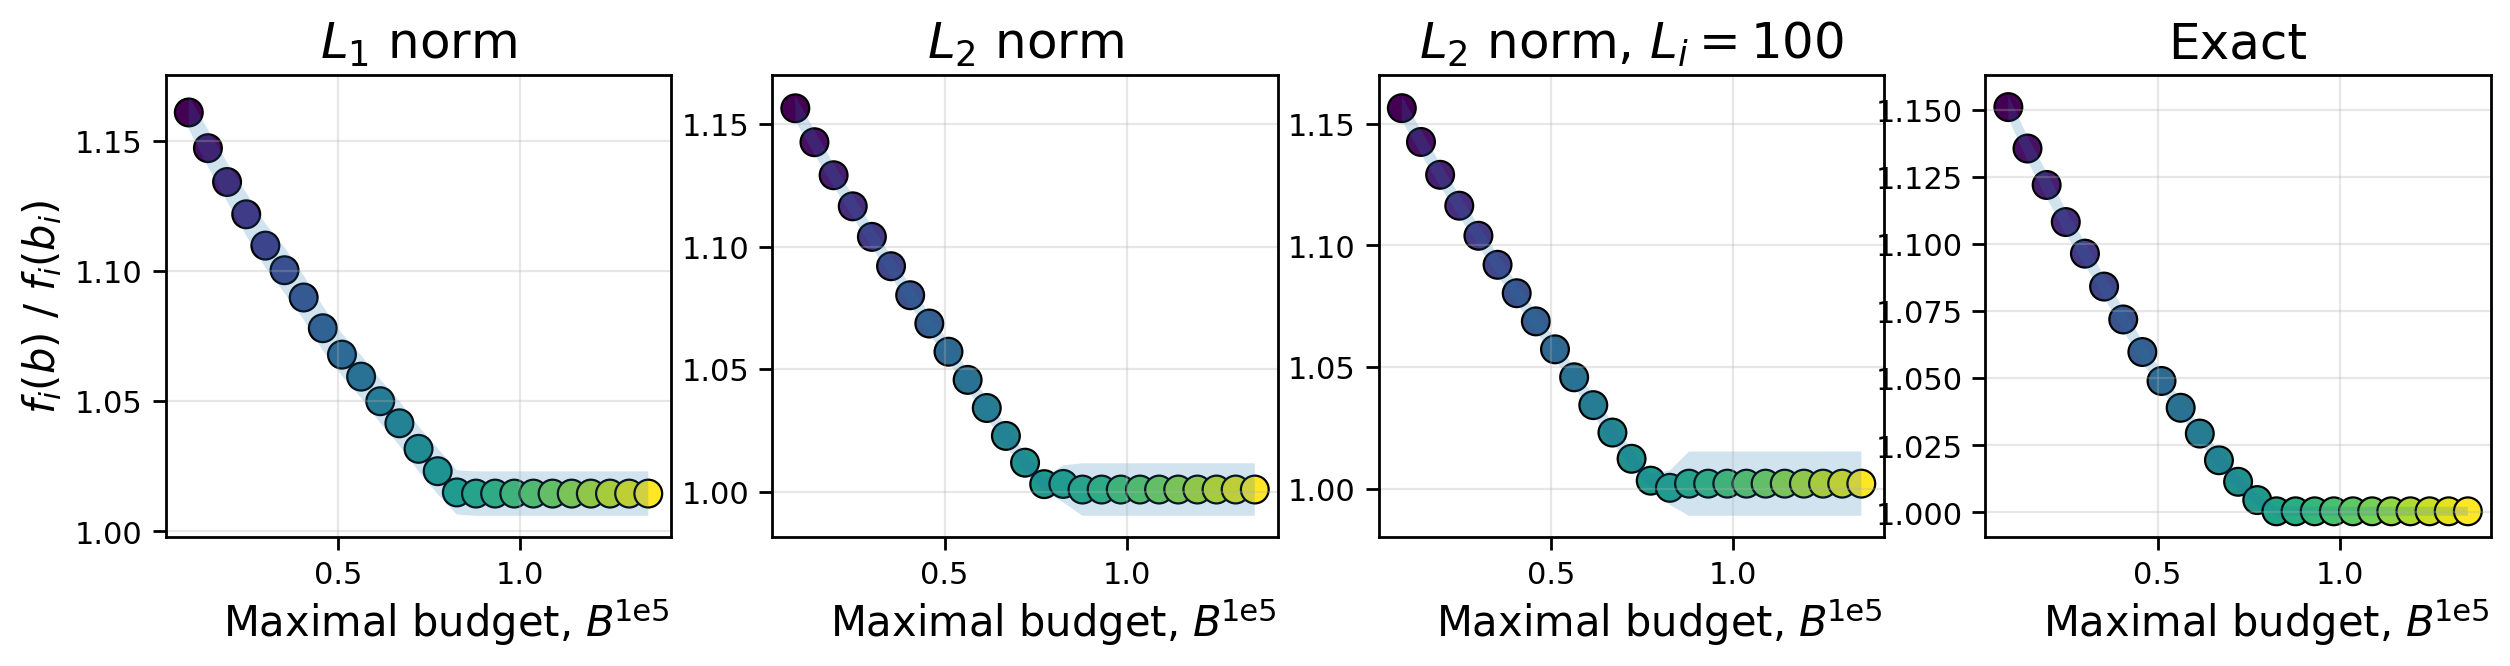
\includegraphics[width=\textwidth]{figures/simplest/relations.png}
            \caption{ Зависимость относительного прироста функции от бюджета для разных способов решения задачи производства.}
    \label{fig:simple:results}
\end{figure}
    
\begin{figure}
    \centering
    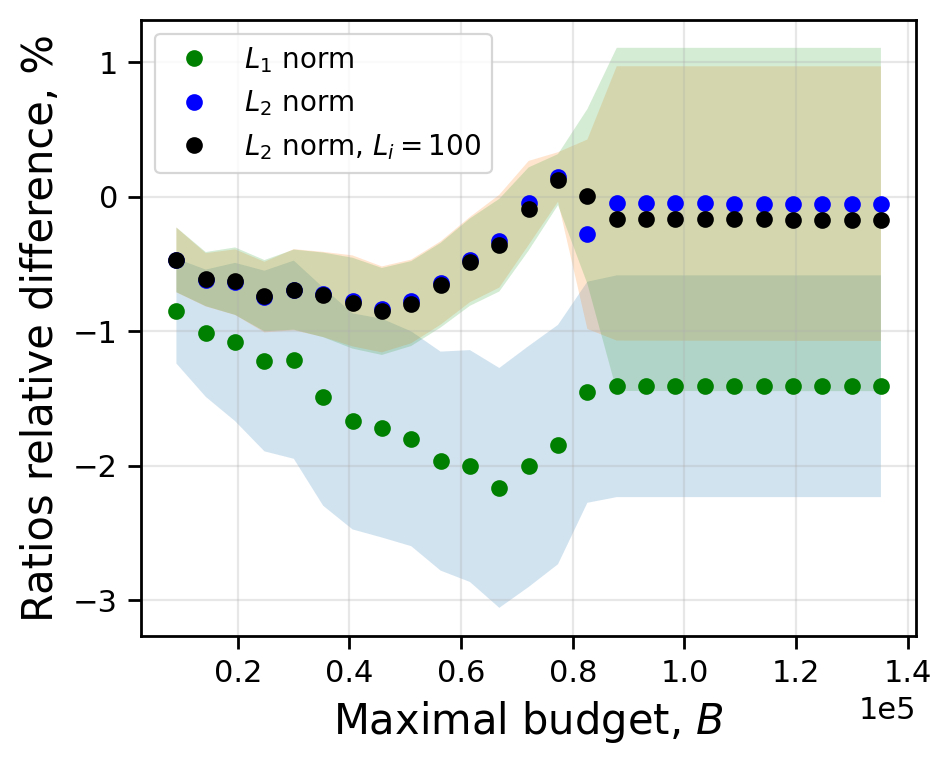
\includegraphics[width=0.5\textwidth]{figures/simplest/relative_difference.png}
    \caption{ Относительная разность качества приближенного решения с качеством точного решения для задачи производства.}
    \label{fig:simple:relations}
\end{figure}

\subsection{Конкурирующие потоки минимальной цены}\label{exp:concurrent}
Задача конкурирующих потоков минимальной цены (minimal cost multicommodity flow, MCF) ставится следующим образом: задан граф $\mathcal{G}(V, E)$, у которого $m$ вершин и $n$ ребер. У ребер $e \in E$  задана пропускная способность $b_e$ и стоимость единицы потока $c_e$ для этой пропускной способности.  Кроме графа заданы потоки, которые необходимо обеспечивать сетью: $(s_i, t_i, f_i)$. Эта тройка означает источник $s$, сток $t$ и требуемый объем потока $f$. Обозначим эти запросы через матрицу корреспонденций $D$: $\forall i: D_{s_i, t_i} = f_i$. Требуется найти потоки в графе  $F \in\mbR^{n\times m}$, которые обеспечат выполнение всех заказов при минимально возможной стоимости.

Задача переписывается в виде задачи линейного программирования \cite{bazaraa2011linear}. Для этого определяем матрицу смежности вершин и ребер $A \in \mbR^{m\times n}$. Каждый столбец содержит ровно два ненулевых значения. Столбец, соответствующий ребру $(i, j)$ содержит "$+1$" в строке  $i$, "$-1$" в строке $j$, и нули во всех других строках. Для каждой вершины вводится вектор поставок  $d_i \in \mbR^m$, он нужен для записи всех потоков, исходящих из этой вершины. При помощи матрицы корреспонденции $D$ компоненты $d_i$ расписываются в виде:
\begin{equation*}
d_{ij} = 
\begin{cases}
    \sum_{k \neq j} D_{ik} & i == j \\
    -d_{ij}
\end{cases}
\end{equation*}

Соединим эти вектор-столбцы в матрицу и обозначим её $D_A \in \mbR^{m\times m}$, эта матрицы используется для удобной записи задачи. 
Используя \cite{bazaraa2011linear}, мы записываем оптимизационную задачу следующим образом:

\begin{align*}
    \min_{F} c_e^T F \textbf{1} & \\
    \text{s.t.} & ~ F\textbf{1} \leq b \\
                & ~ AF = D_A\\
\end{align*}

в этой формулировке задача может не иметь выполнимой точки в силу ограничения с  $b$. Чтобы убрать ограничения по $b$ и сделать задачу проще добавим штраф $y$ к задаче:
\begin{align*}
    \min_{F} c^T F \textbf{1} + c_a^T y & \tag{$MCF$}\label{opt:MCF}\\
    \text{s.t.} & ~ F\textbf{1} \leq b + y\\
                & ~ AF = D_A\\
\end{align*}

Этот штраф интерпретируется как аренда дополнительной пропускной способности в сети. Обозначим $g(b, D) = \text{value}(MCF(b, D))$.

Теперь опишем сценарий использования метода. Есть некая компания, которая предоставляет услугу доставки посылок/сообщений в некой сети. Для работы ей необходимо арендовать полосу пропускания. Она может арендовать полосу пропускания в начале периода по цене $c_b$ и арендовать дополнительную полосу пропускания в течение периода по цене $c_a$. На практике это происходит поэтапно, поскольку она арендуется заранее на длительный срок. В каждый период времени существуют требования на поставки -- матрица корреспонденции $D_i$, потоки из которой необходимо выполнить. Эти матрицы задают сценарии использования сети.  Компании они не известны на момент начала периода. Пусть она в течение $m$ периодов работала с разными арендованными мощностями $b_i$ и пронаблюдала $D_i$. В конце периода она подводит итоги и наблюдает свои расходы внутри периода $f_i(b_i) =g(b_i, D_i)$. Эти функции удовлетворяют условиям Липшица. Необходимо при заданном бюджете закупить пропускную способность так, чтобы она обеспечила небольшие траты для разных ситуаций. Компании на данный момент известны только те $D_i$ которые она пронаблюдала. Тут и появляется необходимость решать задачу \ref{opt:T1}. Ограничения $K = \{b: c_b^T b \leq B\}$.

\subsubsection{Конкурирующие потоки минимальной цены:результаты}

 В эксперименте используем топологию "germany50" ~~ из датасета SNDLib \cite{orlowski2010sndlib}. Это сеть из 50 вершин и 176 ребер. В датасете совместно с самим графом приводится набор матриц корреспонденции и стоимостей потоков в ребрах. Эти матрицы будут использованы в качестве матриц $D$. Для решаемости задачи при меньших пропускных способностях провели разреживание запросов: с вероятностью $0.4$ ячейка в матрице обнуляется. Параметры для экспериментов генерировались следующим образом: стоимости потоков $c$ есть в самих графах. На их основе генерировались начальная стоимость аренды и стоимость аренды внутри периода. Если пропускная способность стоит дешевле, то это более качественная пропускная полоса, поэтому стоимость такой полосы должна быть выше. Также считаем аренду дороже, чем обслуживание. Поэтому стоимости в начале периода генерировались как $(c_b)_i = (1/\sqrt{c_i}) \xi$, где $\xi \sim U[9, 11]$. Стоимость аренды во время периода считаем выше: $(c_a)_i = (c_b)_i * \xi, \sim U[1.05, 1.15]$, то есть дороже от 5 до 15%. 

Для этой задачи точное решение задачи найти не удалось, так как решатель не сошелся. Рассмотрели нормы $\|\cdot\|_1$; $\|\cdot\|_2$; $\|\cdot\|_\infty$. Рисунок \ref{fig:mcf:relations}  показывает относительный прирост значений функций при разных значениях бюджета. Точка это усреднение отношений значений функций к значениям в изначальных точках. Закрашенная область -- $\pm$ дисперсия. По картинкам видно, что $\|\cdot\|_\infty$ работает хуже остальных. 

Так как для этого случая нет точного решения, сравним эти решения с средним качеством решения. Это показано на рисунке \ref{fig:mcf:relative_diff}. Больше значение -- лучше. Видим, что разные нормы лучше работают для разных бюджетов: $L_1$ норма выдает разреженные решения, они не оптимальны для небольших бюджетов, поскольку некоторые ресурсы мало покупаются, но хорошо для большого бюджета, поскольку лишние ресурсы покупаются самые дешевые. $L_2$ норма получает решение, которое до 10\% лучше среднего качества решения. Аналогично $L_1$, но уже на больших бюджетах. 

\begin{figure}
\centering
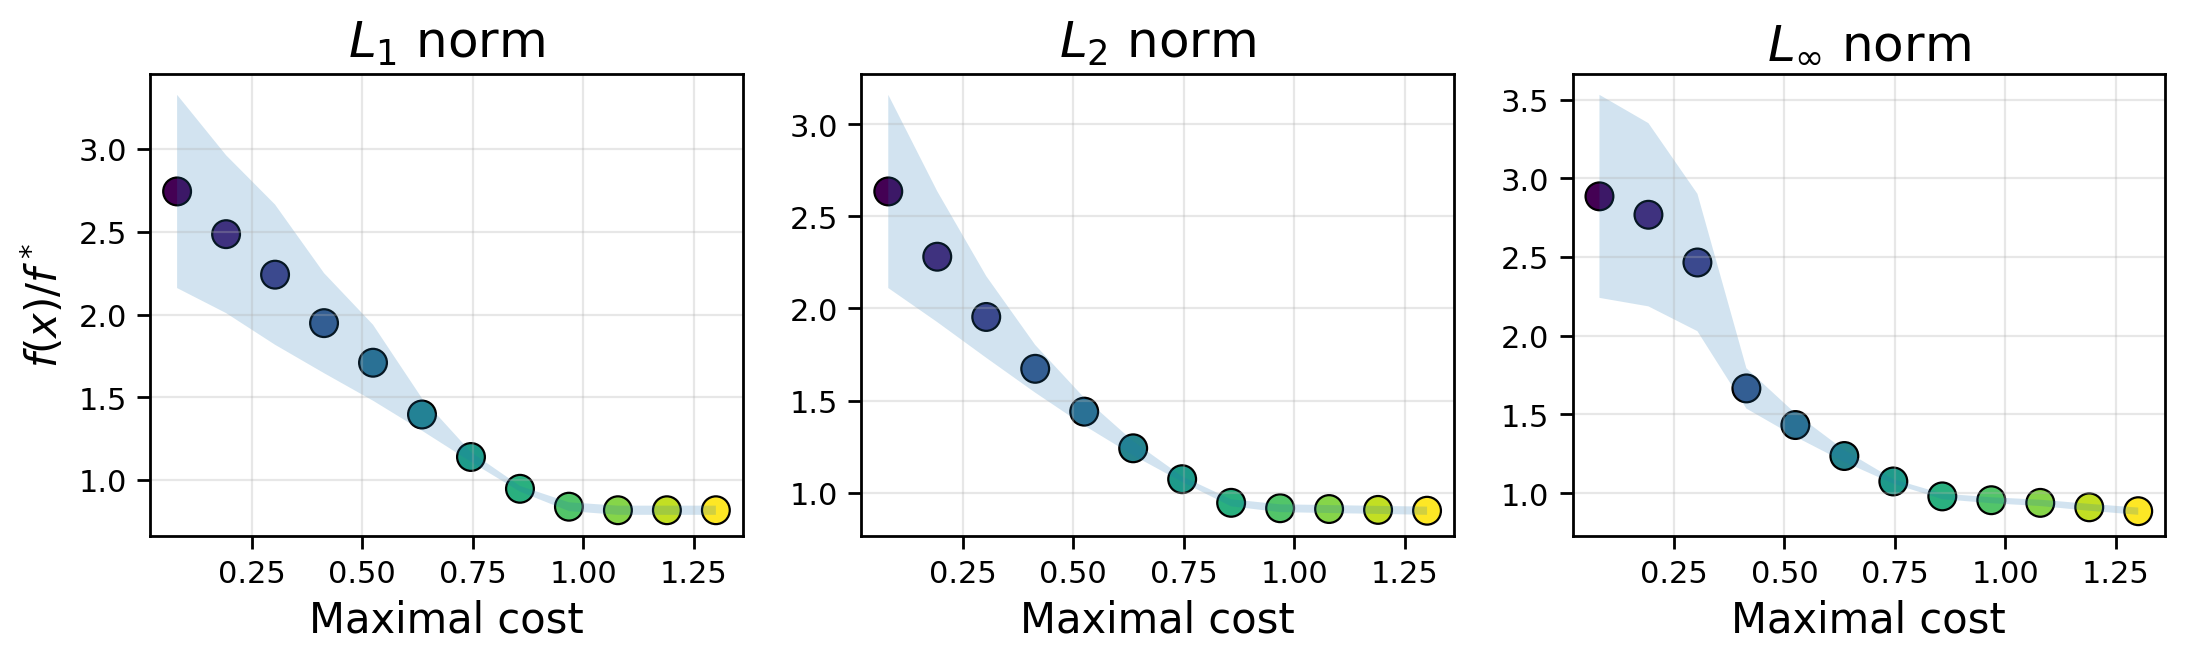
\includegraphics[width=\textwidth]{figures/mcf/relations.png}
            \caption{ Зависимость относительного прироста функции в зависимости от бюджета для разных способов решения задачи MCF.}
\label{fig:mcf:relations}
\end{figure}
    
\begin{figure}
    \centering
    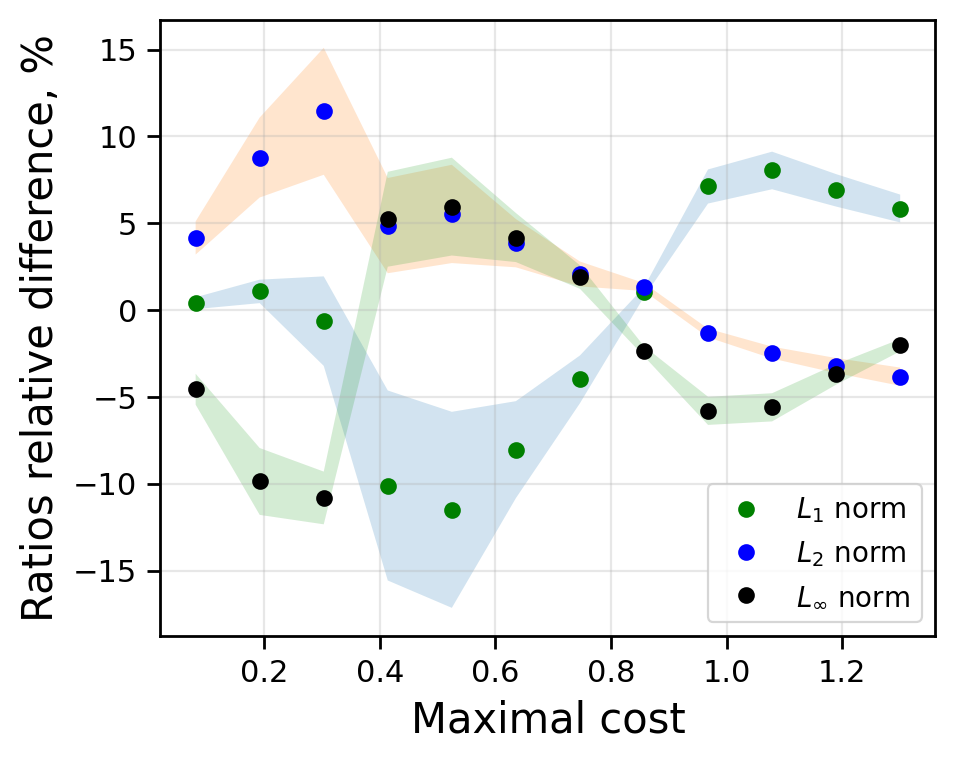
\includegraphics[width=0.5\textwidth]{figures/mcf/relative_difference.png}
    \caption{ Относительная разность качеств приближенного решения со средним качеством решения для задачи MCF.}
    \label{fig:mcf:relative_diff}
\end{figure}



\newpage
\section{Выводы}
В работе предложен метод скаляризации, не требующий подбора гиперпараметров, который представляет собой обобщение понятия конкурентного решения. Мы также показали связь нашего метода скаляризации с подходом, предложенным в \cite{gembicki1975approach}.

Для случая Липшицевых функций мы представили метод приближенного решения задачи оптимизации. Этот метод особенно полезен в случаях, когда вычисления функций являются дорогими, так как он работает только с заранее вычисленным набором значений. Необходимость таких методов обусловлена масштабами современных задач, например, в области оптимизации топологии телевизионных сетей и сетей поставок. Проведенные эксперименты продемонстрировали эффективность и практическую полезность предложенного метода, подтверждая его применимость в разных сценариях.
\newpage
\bibliographystyle{unsrt}
\bibliography{biblio}
\end{document} 